\section{Experiment design}

\begin{figure}
	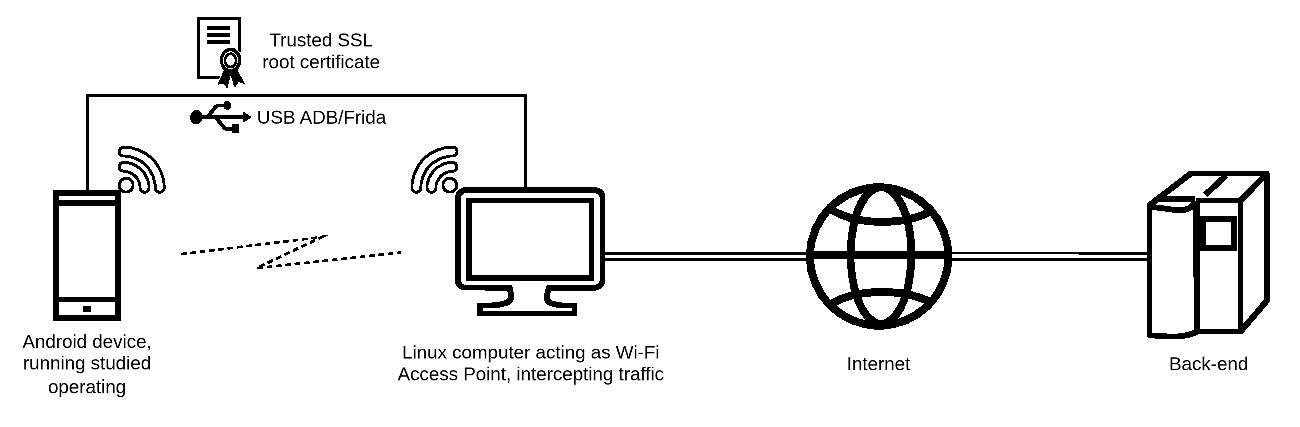
\includegraphics[width=\textwidth]{images/devices.eps}
	\caption{Measurement setup. Android device running studied operating systems is configured to access Internet using Wi-Fi. Access point is hosted on a Linux computer, running traffic interception and capturing software. Custom system certificate is installed on the phone using root access. USB connection is used for ADB/Frida communication.} \label{fig1}
\end{figure}

\subsection{Measurement Scenarios}
To enable consistent, comparable measurements across Android distributions, four setup scenarios were defined. Each scenario specifies (i) Google account state, (ii) consent/permission posture, and (iii) what Google components are present. Not all scenarios apply to every operating system due to their characteristics.

\paragraph{Scenario A: Minimal Setup, No Google Account.}
The device is configured with a maximum privacy in mind, avoiding Google account sign-in. During initial setup, only strictly required prompts are accepted, optional data-sharing is declined.

\paragraph{Scenario B: Minimal Setup, With Google Account.}
This scenario mirrors \textit{Scenario A} in all consent and permission choices, but includes login into Google account during initial setup (or immediately after). Google account used in this scenario has settings adjusted toward minimal data collection.

\paragraph{Scenario C: Default Setup, With Google Account.}
The device is configured to reflect a typical user path. Google account sign-in is performed and default recommendations are accepted (including prompted permissions).

\paragraph{Scenario D: Extremely Minimal Setup, No Google Components.}
This scenario is possible only on systems that do not bundle/enable Google components/replacements by default.

[Scenario adaptation to microg/graphene...]